\documentclass{article}\usepackage[]{graphicx}\usepackage[]{color}
%% maxwidth is the original width if it is less than linewidth
%% otherwise use linewidth (to make sure the graphics do not exceed the margin)
\makeatletter
\def\maxwidth{ %
  \ifdim\Gin@nat@width>\linewidth
    \linewidth
  \else
    \Gin@nat@width
  \fi
}
\makeatother

\definecolor{fgcolor}{rgb}{0.345, 0.345, 0.345}
\newcommand{\hlnum}[1]{\textcolor[rgb]{0.686,0.059,0.569}{#1}}%
\newcommand{\hlstr}[1]{\textcolor[rgb]{0.192,0.494,0.8}{#1}}%
\newcommand{\hlcom}[1]{\textcolor[rgb]{0.678,0.584,0.686}{\textit{#1}}}%
\newcommand{\hlopt}[1]{\textcolor[rgb]{0,0,0}{#1}}%
\newcommand{\hlstd}[1]{\textcolor[rgb]{0.345,0.345,0.345}{#1}}%
\newcommand{\hlkwa}[1]{\textcolor[rgb]{0.161,0.373,0.58}{\textbf{#1}}}%
\newcommand{\hlkwb}[1]{\textcolor[rgb]{0.69,0.353,0.396}{#1}}%
\newcommand{\hlkwc}[1]{\textcolor[rgb]{0.333,0.667,0.333}{#1}}%
\newcommand{\hlkwd}[1]{\textcolor[rgb]{0.737,0.353,0.396}{\textbf{#1}}}%

\usepackage{framed}
\makeatletter
\newenvironment{kframe}{%
 \def\at@end@of@kframe{}%
 \ifinner\ifhmode%
  \def\at@end@of@kframe{\end{minipage}}%
  \begin{minipage}{\columnwidth}%
 \fi\fi%
 \def\FrameCommand##1{\hskip\@totalleftmargin \hskip-\fboxsep
 \colorbox{shadecolor}{##1}\hskip-\fboxsep
     % There is no \\@totalrightmargin, so:
     \hskip-\linewidth \hskip-\@totalleftmargin \hskip\columnwidth}%
 \MakeFramed {\advance\hsize-\width
   \@totalleftmargin\z@ \linewidth\hsize
   \@setminipage}}%
 {\par\unskip\endMakeFramed%
 \at@end@of@kframe}
\makeatother

\definecolor{shadecolor}{rgb}{.97, .97, .97}
\definecolor{messagecolor}{rgb}{0, 0, 0}
\definecolor{warningcolor}{rgb}{1, 0, 1}
\definecolor{errorcolor}{rgb}{1, 0, 0}
\newenvironment{knitrout}{}{} % an empty environment to be redefined in TeX

\usepackage{alltt}
\usepackage[margin=1.1in]{geometry}
\usepackage{setspace}
\usepackage{amssymb, amsmath}
\usepackage{graphicx}
\usepackage{wrapfig}
\usepackage{subcaption}
\usepackage{float}

\usepackage{hyperref}
\hypersetup{
    colorlinks=true,
    linkcolor=blue,
    filecolor=magenta,      
    urlcolor=cyan,
}
\IfFileExists{upquote.sty}{\usepackage{upquote}}{}
\begin{document}



\title{Quantitative Assesment for Gelber Group}
\author{Riley Robertson}
\maketitle

\section{Scope}
This report aims to develop and explain a pricing model for the Global X MSCI Greece ETF (GREK). The model will price the close value of the fund for any business day since its inception. The data used is mostly macroeconomic, like market volumes and exchange rates. I initially tried to search for securities not held by the fund that were highly correlated to the fund or to some of its largest holdings, but I was unable to find any significant relations in that search (exlcuding depository receipts). Unfortunately, many macroeconomic variables like imports/exports, unemployment, GDP, and consumer price infex were only available on a yearly basis, so they were not of much use when trying to price by the day.

\section{Findings}
After combing through all of the data available, I decided to use solely the USD-Euro exchange rate. I certainly would've liked to build a more sophisticated and robust model, but I was unable to acquire sufficient data (details in ``Scope'' section above). The relation betwee GREK's closing price and the exchange rate appears to be non-linear, but neither a $\log$ nor a square-root transform made a significant difference in the correlation between the two variables.
\begin{figure}[h]
\centering
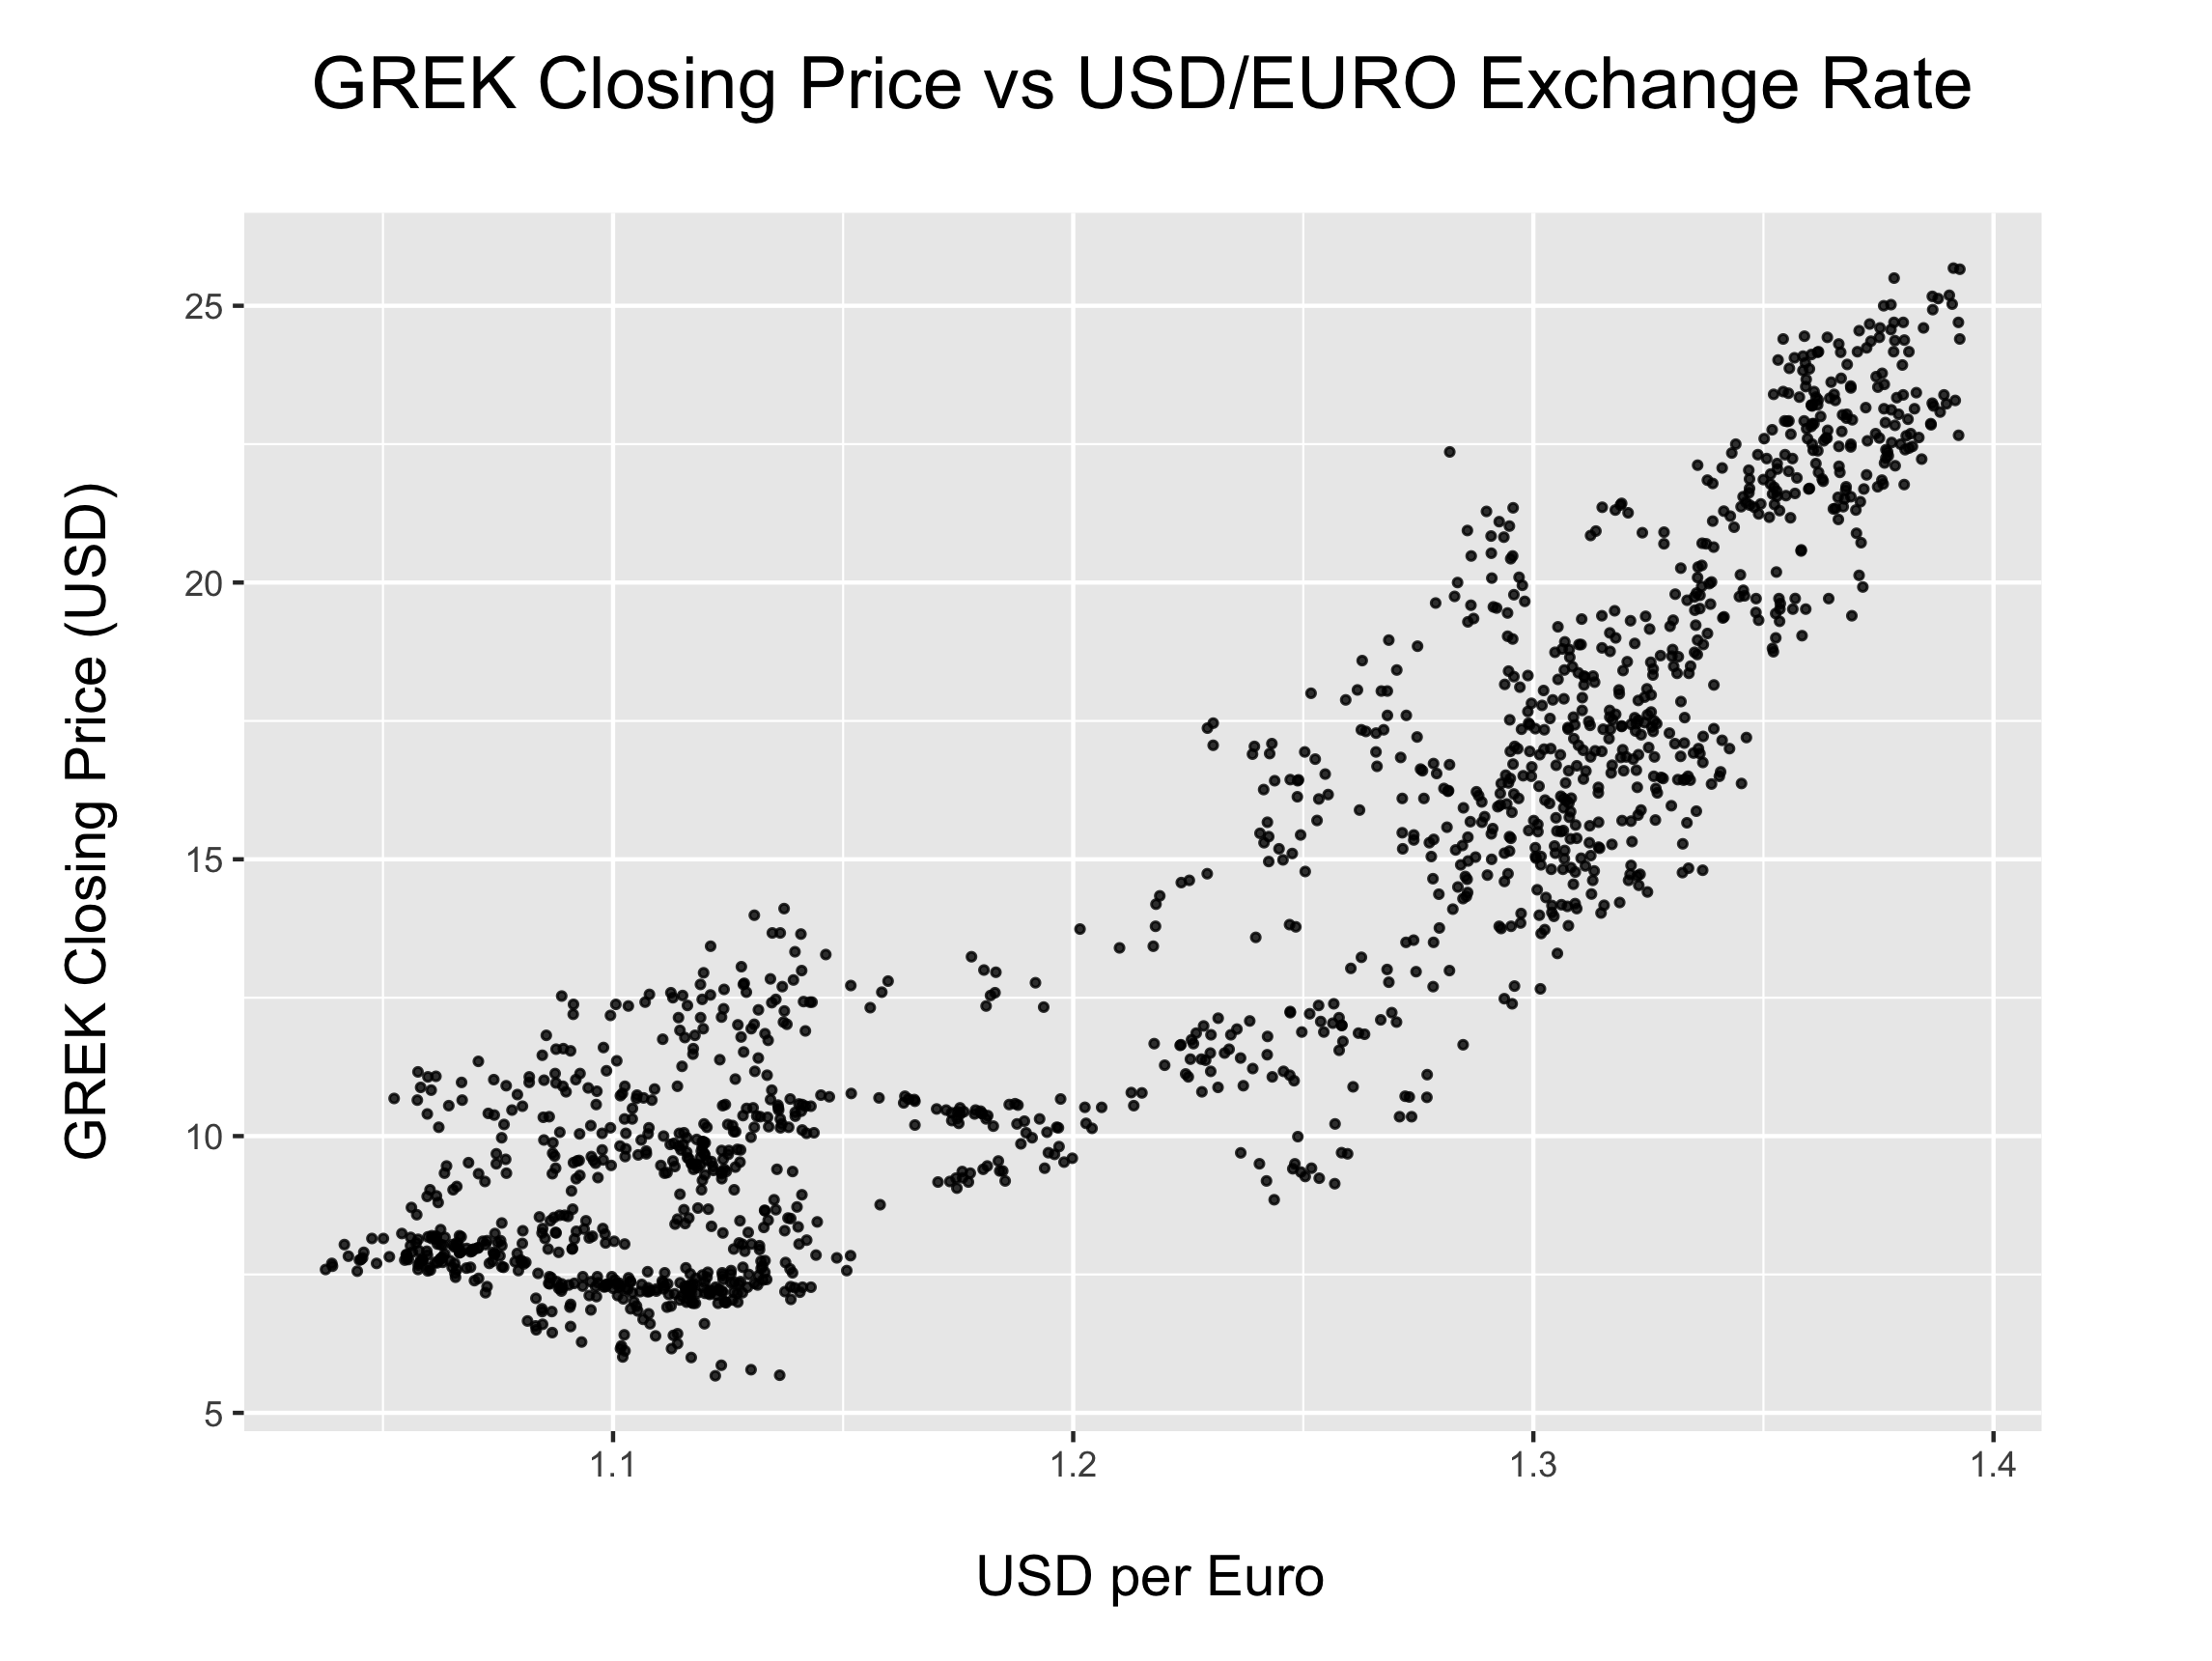
\includegraphics[width=0.6\textwidth]{figures/close_vs_ex_rate.png}
\caption{GREK Closing Price vs USD/EURO Exchange Rate}
\end{figure}


\begin{knitrout}
\definecolor{shadecolor}{rgb}{0.969, 0.969, 0.969}\color{fgcolor}\begin{kframe}
\begin{alltt}
\hlkwd{cor}\hlstd{(data}\hlopt{$}\hlstd{close, data}\hlopt{$}\hlstd{ex_rate)}
\end{alltt}
\begin{verbatim}
## [1] 0.9100587
\end{verbatim}
\begin{alltt}
\hlkwd{cor}\hlstd{(}\hlkwd{log}\hlstd{(data}\hlopt{$}\hlstd{close), data}\hlopt{$}\hlstd{ex_rate)}
\end{alltt}
\begin{verbatim}
## [1] 0.9126452
\end{verbatim}
\begin{alltt}
\hlkwd{cor}\hlstd{(}\hlkwd{sqrt}\hlstd{(data}\hlopt{$}\hlstd{close), data}\hlopt{$}\hlstd{ex_rate)}
\end{alltt}
\begin{verbatim}
## [1] 0.9151675
\end{verbatim}
\end{kframe}
\end{knitrout}

With that observation, I decided on running a LOESS local regression. This model had a surprisingly good fit

\begin{figure}[h]
\centering
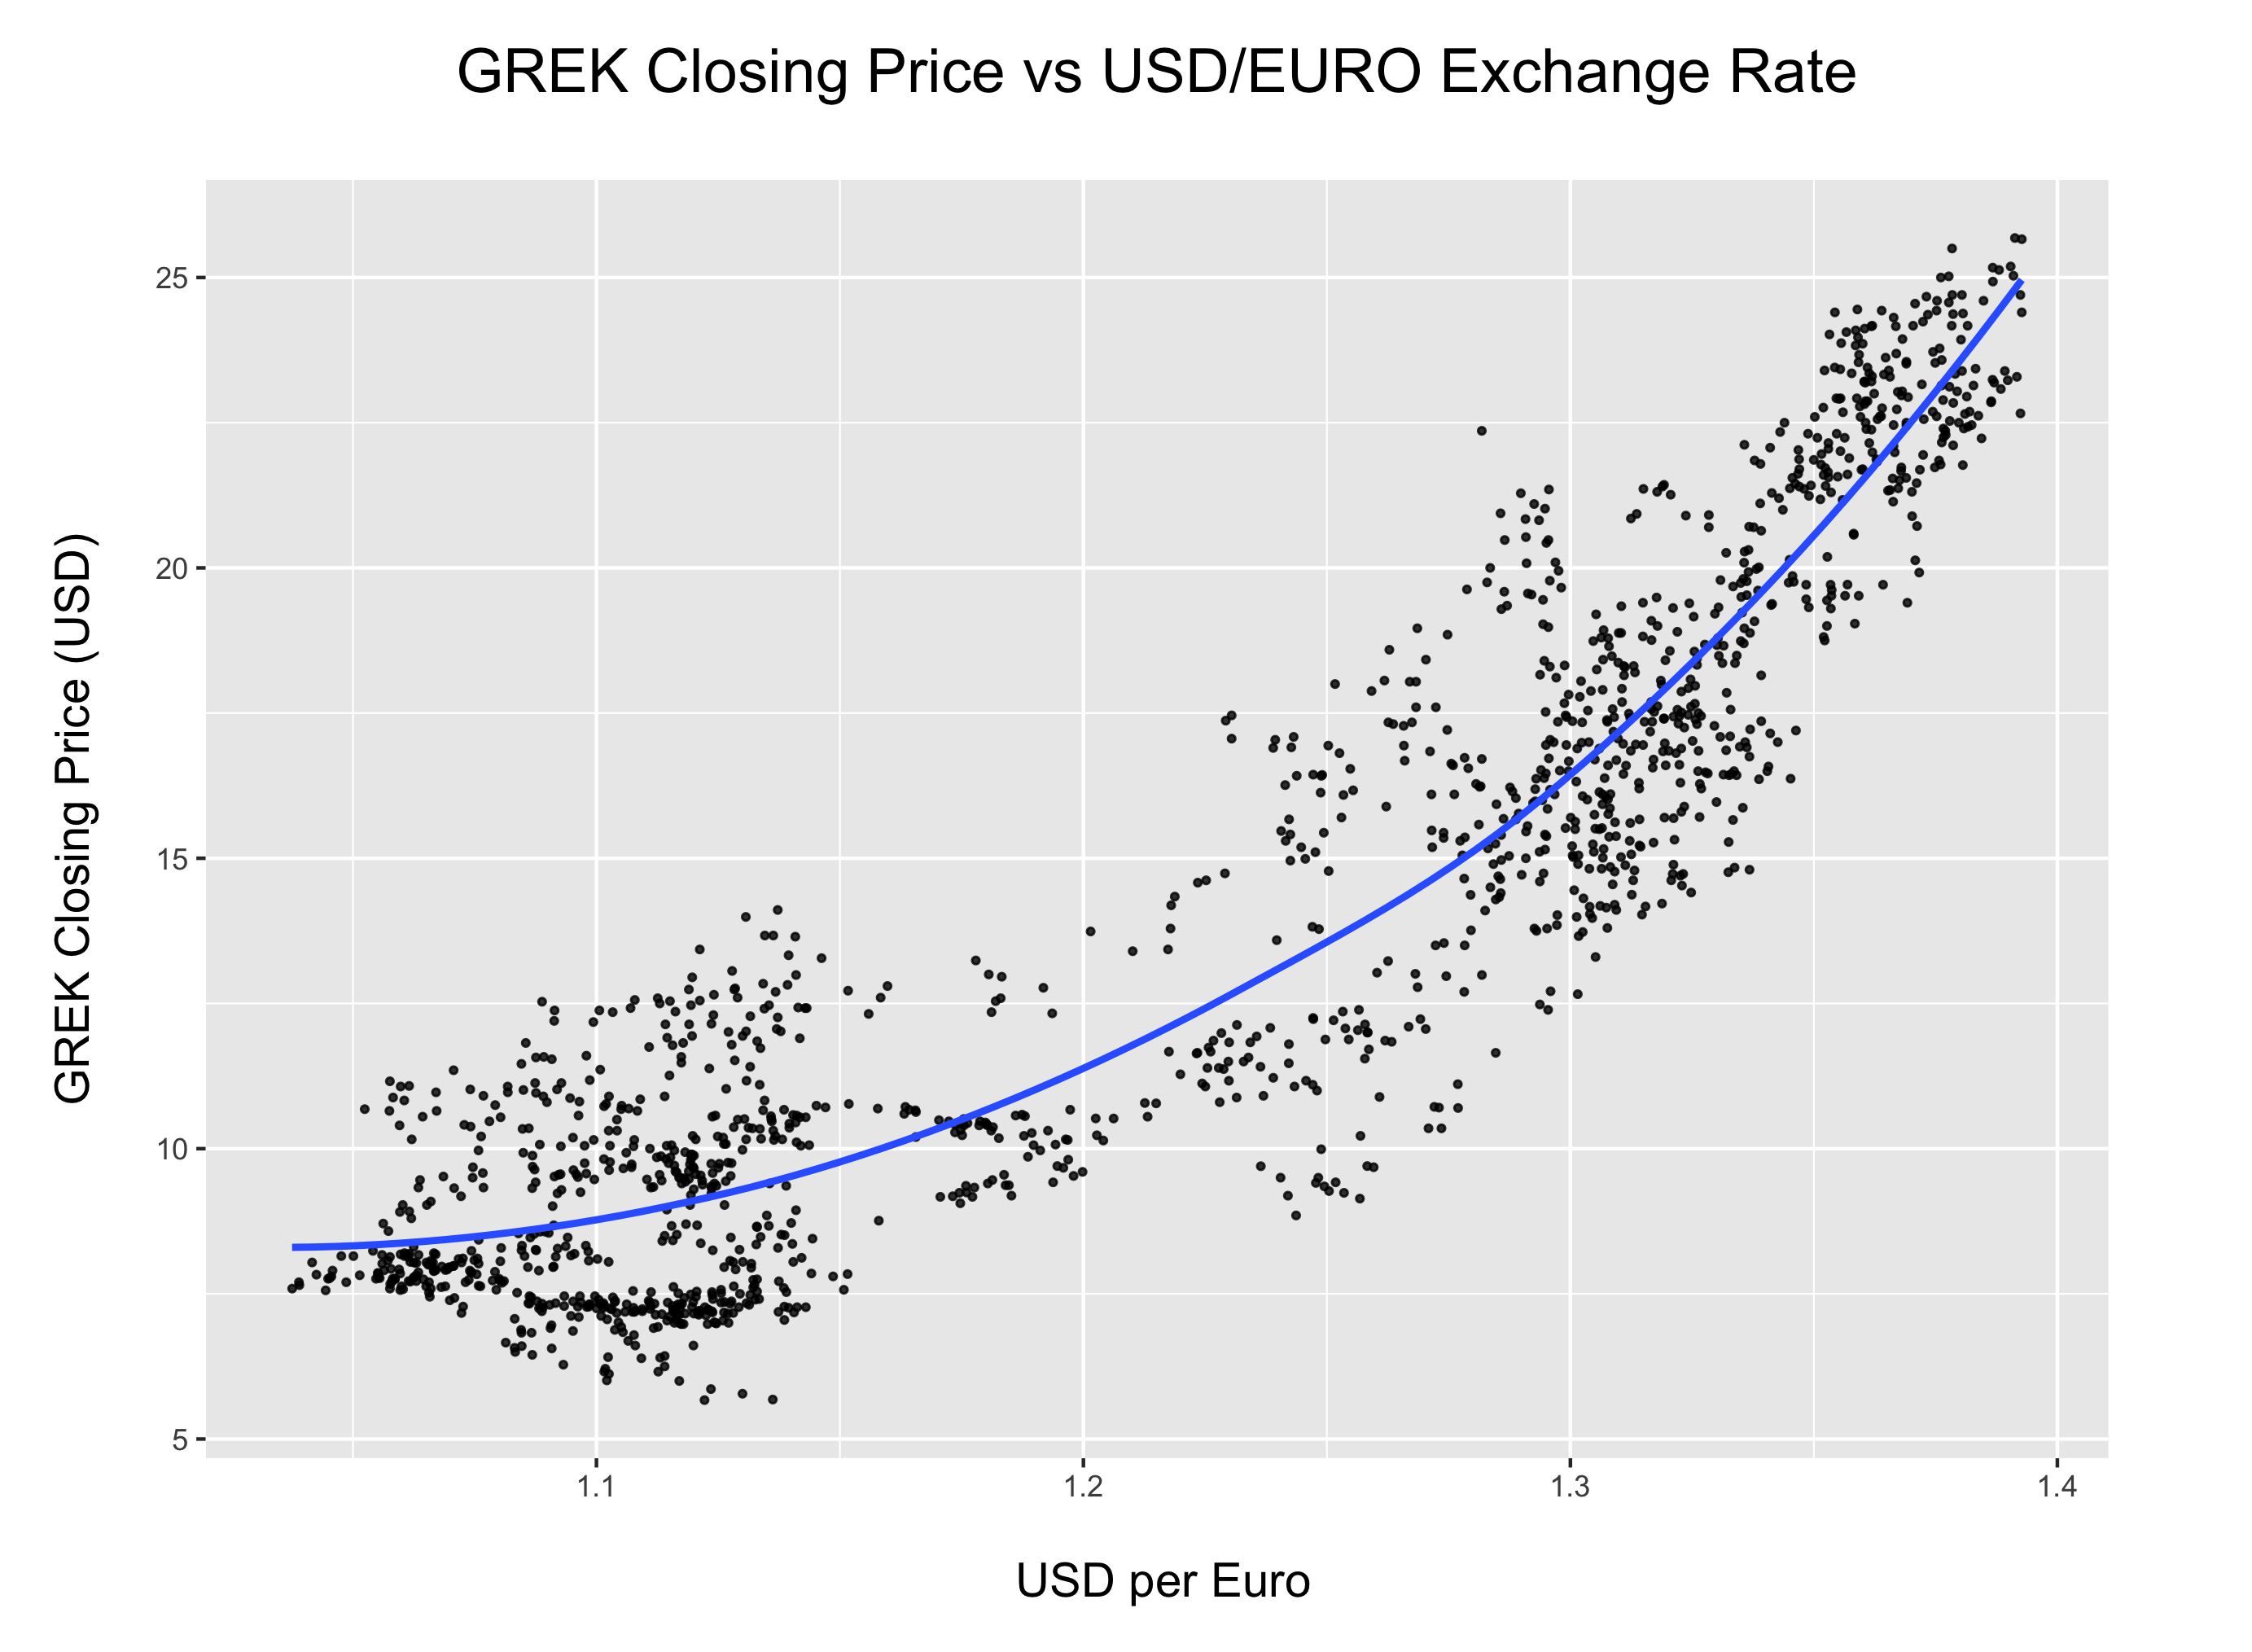
\includegraphics[width=0.6\textwidth]{figures/close_vs_ex_rate_loess.png}
\caption{GREK Closing Price vs USD/EURO Exchange Rate}
\end{figure}

I say it's ``surprisingly good'' because it's based on just one explanatory variable, and it has the following fit metrics:
\begin{knitrout}
\definecolor{shadecolor}{rgb}{0.969, 0.969, 0.969}\color{fgcolor}\begin{kframe}
\begin{alltt}
\hlcom{# The expected difference from the close price and the model is near 0}
\hlkwd{mean}\hlstd{(data}\hlopt{$}\hlstd{close} \hlopt{-}  \hlstd{data}\hlopt{$}\hlstd{loess_prediction)}
\end{alltt}
\begin{verbatim}
## [1] -0.01125454
\end{verbatim}
\begin{alltt}
\hlcom{# This model predicts ~88% of variation in close price}
\hlkwd{cor}\hlstd{(data}\hlopt{$}\hlstd{close, data}\hlopt{$}\hlstd{loess_prediction)}\hlopt{^}\hlnum{2}
\end{alltt}
\begin{verbatim}
## [1] 0.8786443
\end{verbatim}
\end{kframe}
\end{knitrout}

Because LOESS is non-parametric, we cannot write down what the model is. However, the supplied code allows one to price at any given time $t$ by finding the exchange rate at $t$ and then seeing what the predicted value of GREK's closing price is at that exchange rate.
\begin{knitrout}
\definecolor{shadecolor}{rgb}{0.969, 0.969, 0.969}\color{fgcolor}\begin{kframe}
\begin{alltt}
\hlkwd{prediction}\hlstd{(}\hlstr{"2012/01/02"}\hlstd{)}
\end{alltt}
\begin{verbatim}
## [1] 16.88624
\end{verbatim}
\end{kframe}
\end{knitrout}
The ``YYYY/MM/DD'' format must be used, but the given day need not be a business day (the model will predict on the first business day that comes after the inputted day)

\section{Conclusion}
Admittedly, this model is very simple. As I've said, this is due in largest part to the fact that I had difficulty getting relevant data that was collected daily. Some next steps to improve this model would be to consider more macroeconomic factors as well as use the prices of other securities to predict the price of GREK.


\section{Appendix}
Here is all of the R code that I've used for this project. The datasets I used can be found on \href{https://github.com/jrr8/Gelber}{my GitHub}.

\begin{knitrout}
\definecolor{shadecolor}{rgb}{0.969, 0.969, 0.969}\color{fgcolor}\begin{kframe}
\begin{alltt}
\hlcom{# adding dependencies}
\hlkwd{library}\hlstd{(Quandl)}
\hlkwd{library}\hlstd{(ggplot2)}
\hlkwd{Quandl.api_key}\hlstd{(}\hlstr{"sfk1toiCxwvhsvgMwwFe"}\hlstd{)}

\hlcom{# reading the data in}
\hlstd{grek} \hlkwb{<-} \hlkwd{read.csv}\hlstd{(}\hlstr{"data/GREK_2yrs.csv"}\hlstd{)}
\hlstd{ex_rates} \hlkwb{<-} \hlkwd{Quandl}\hlstd{(}\hlstr{"FED/RXI_US_N_B_EU"}\hlstd{,} \hlkwc{start_date}\hlstd{=}\hlstr{"2011-12-07"}\hlstd{)}

\hlcom{# cleaning into the formats we'd like}
\hlstd{grek}\hlopt{$}\hlstd{volume} \hlkwb{<-} \hlkwd{as.vector}\hlstd{(grek}\hlopt{$}\hlstd{volume)}
\hlstd{grek} \hlkwb{<-} \hlstd{grek[}\hlnum{2}\hlopt{:}\hlkwd{nrow}\hlstd{(grek),]}
\hlstd{grek} \hlkwb{<-} \hlstd{grek[}\hlkwd{order}\hlstd{(grek}\hlopt{$}\hlstd{date),]}
\hlstd{grek}\hlopt{$}\hlstd{Month} \hlkwb{<-} \hlkwd{paste}\hlstd{(}\hlkwd{substr}\hlstd{(grek}\hlopt{$}\hlstd{date,} \hlnum{1}\hlstd{,} \hlnum{4}\hlstd{),} \hlkwd{substr}\hlstd{(grek}\hlopt{$}\hlstd{date,} \hlnum{6}\hlstd{,} \hlnum{7}\hlstd{),} \hlkwc{sep} \hlstd{=} \hlstr{"-"}\hlstd{)}
\hlstd{ex_rates}\hlopt{$}\hlstd{date} \hlkwb{<-} \hlkwd{format}\hlstd{(ex_rates}\hlopt{$}\hlstd{Date,} \hlkwc{format} \hlstd{=} \hlstr{"%Y/%m/%d"}\hlstd{)}
\hlkwd{names}\hlstd{(ex_rates)[}\hlkwd{names}\hlstd{(ex_rates)} \hlopt{==} \hlstr{"Value"}\hlstd{]} \hlkwb{<-} \hlstr{"ex_rate"}

\hlcom{# looking at exchange rate}
\hlstd{data} \hlkwb{<-} \hlkwd{merge}\hlstd{(grek, ex_rates,} \hlkwc{by.x} \hlstd{=} \hlstr{"date"}\hlstd{)}
\hlstd{lo} \hlkwb{<-} \hlkwd{loess}\hlstd{(data}\hlopt{$}\hlstd{close} \hlopt{~} \hlstd{data}\hlopt{$}\hlstd{ex_rate,} \hlkwc{model} \hlstd{=} \hlnum{TRUE}\hlstd{)}
\hlstd{data}\hlopt{$}\hlstd{loess_prediction} \hlkwb{<-} \hlkwd{predict}\hlstd{(lo,} \hlkwd{data.frame}\hlstd{(}\hlkwc{close} \hlstd{=} \hlkwd{seq}\hlstd{(}\hlnum{5}\hlstd{,} \hlnum{25}\hlstd{,} \hlkwc{length.out} \hlstd{=} \hlkwd{nrow}\hlstd{(data))))}

\hlstd{prediction} \hlkwb{<-} \hlkwa{function}\hlstd{(}\hlkwc{x}\hlstd{) \{}
  \hlkwa{while} \hlstd{(}\hlkwd{nrow}\hlstd{(data[data}\hlopt{$}\hlstd{date} \hlopt{==} \hlstd{x, ])} \hlopt{==} \hlnum{0}\hlstd{) \{}
    \hlkwa{if} \hlstd{(}\hlkwd{substr}\hlstd{(x,} \hlkwd{nchar}\hlstd{(x),} \hlkwd{nchar}\hlstd{(x))} \hlopt{!=} \hlstr{"9"}\hlstd{) \{}
      \hlstd{x} \hlkwb{<-} \hlkwd{paste}\hlstd{(}\hlkwd{substr}\hlstd{(x,} \hlnum{1}\hlstd{,} \hlkwd{nchar}\hlstd{(x)} \hlopt{-} \hlnum{1}\hlstd{),}
                 \hlkwd{as.numeric}\hlstd{(}\hlkwd{substr}\hlstd{(x,} \hlkwd{nchar}\hlstd{(x),} \hlkwd{nchar}\hlstd{(x)))} \hlopt{+} \hlnum{1}\hlstd{,} \hlkwc{sep}\hlstd{=}\hlstr{""}\hlstd{)}
    \hlstd{\}} \hlkwa{else} \hlstd{\{}
      \hlstd{x} \hlkwb{<-} \hlkwd{paste}\hlstd{(}\hlkwd{substr}\hlstd{(x,} \hlnum{1}\hlstd{,} \hlkwd{nchar}\hlstd{(x)} \hlopt{-} \hlnum{2}\hlstd{),}
                 \hlkwd{as.numeric}\hlstd{(}\hlkwd{substr}\hlstd{(x,} \hlkwd{nchar}\hlstd{(x)} \hlopt{-} \hlnum{1}\hlstd{,} \hlkwd{nchar}\hlstd{(x)} \hlopt{-} \hlnum{1}\hlstd{))} \hlopt{+} \hlnum{1}\hlstd{,} \hlnum{0}\hlstd{,} \hlkwc{sep}\hlstd{=} \hlstr{""}\hlstd{)}
    \hlstd{\}}
  \hlstd{\}}
  \hlkwd{return}\hlstd{(lo}\hlopt{$}\hlstd{fitted[}\hlkwd{which}\hlstd{(data}\hlopt{$}\hlstd{date} \hlopt{==} \hlstd{x)])}
\hlstd{\}}
\end{alltt}
\end{kframe}
\end{knitrout}


\end{document}
